% Author: Xu Chen, University of Washington
% Lab 01 scene: heater-and-sensor board A (demo) on a bench, and its control problem.
\documentclass[border=4pt]{standalone}
% Author: Xu Chen, University of Washington
% Shared TikZ style for the Control in Practice scene figures. % Author: Xu Chen, University of Washington
% Shared TikZ style for the Control in Practice scene figures. % Author: Xu Chen, University of Washington
% Shared TikZ style for the Control in Practice scene figures. \input{../../../docs/figures/cipstyle} from a lab.
\usepackage{amsmath,amssymb}
\usepackage[T1]{fontenc}
\usepackage{lmodern}
\usepackage{tikz}
\usepackage[siunitx]{circuitikz}
\usetikzlibrary{arrows.meta,calc,positioning,decorations.pathmorphing,decorations.markings,patterns,shapes.geometric,shadings,fit,backgrounds}
% restrained palette
\definecolor{ink}{HTML}{1A1A1A}
\definecolor{steel}{HTML}{8C96A0}
\definecolor{metal}{HTML}{D5DAE0}
\definecolor{accent}{HTML}{1F4E79}   % controller, signals we choose
\definecolor{plantc}{HTML}{FBE7D6}   % plant fill
\definecolor{sensorc}{HTML}{DCE8F3}  % sensor fill
\definecolor{dist}{HTML}{B03A2E}     % disturbances, forces from the environment
\definecolor{act}{HTML}{2E7D4F}      % actuation
\definecolor{note}{HTML}{555555}
\tikzset{
  every picture/.style={line width=0.8pt, >={Stealth[length=2.4mm]}, font=\small},
  thin line/.style={line width=0.5pt},
  thick line/.style={line width=1.2pt},
  dim/.style={thin line, note, {Stealth[length=1.6mm]}-{Stealth[length=1.6mm]}},
  ground/.style={pattern=north east lines, pattern color=steel, draw=none},
  block/.style={draw=ink, rounded corners=1.5pt, minimum height=9mm, minimum width=16mm, align=center, fill=white},
  plant/.style={block, fill=plantc},
  sensor/.style={block, fill=sensorc},
  ctrl/.style={block, draw=accent, text=accent, thick line},
  sum/.style={draw=ink, circle, minimum size=5mm, inner sep=0pt},
  sig/.style={->, ink},
  distsig/.style={->, dist, thick line},
  force/.style={-{Stealth[length=3mm]}, thick line},
  panel title/.style={font=\normalsize\bfseries, anchor=west, ink},
  caption/.style={font=\footnotesize, note, align=left},
}
 from a lab.
\usepackage{amsmath,amssymb}
\usepackage[T1]{fontenc}
\usepackage{lmodern}
\usepackage{tikz}
\usepackage[siunitx]{circuitikz}
\usetikzlibrary{arrows.meta,calc,positioning,decorations.pathmorphing,decorations.markings,patterns,shapes.geometric,shadings,fit,backgrounds}
% restrained palette
\definecolor{ink}{HTML}{1A1A1A}
\definecolor{steel}{HTML}{8C96A0}
\definecolor{metal}{HTML}{D5DAE0}
\definecolor{accent}{HTML}{1F4E79}   % controller, signals we choose
\definecolor{plantc}{HTML}{FBE7D6}   % plant fill
\definecolor{sensorc}{HTML}{DCE8F3}  % sensor fill
\definecolor{dist}{HTML}{B03A2E}     % disturbances, forces from the environment
\definecolor{act}{HTML}{2E7D4F}      % actuation
\definecolor{note}{HTML}{555555}
\tikzset{
  every picture/.style={line width=0.8pt, >={Stealth[length=2.4mm]}, font=\small},
  thin line/.style={line width=0.5pt},
  thick line/.style={line width=1.2pt},
  dim/.style={thin line, note, {Stealth[length=1.6mm]}-{Stealth[length=1.6mm]}},
  ground/.style={pattern=north east lines, pattern color=steel, draw=none},
  block/.style={draw=ink, rounded corners=1.5pt, minimum height=9mm, minimum width=16mm, align=center, fill=white},
  plant/.style={block, fill=plantc},
  sensor/.style={block, fill=sensorc},
  ctrl/.style={block, draw=accent, text=accent, thick line},
  sum/.style={draw=ink, circle, minimum size=5mm, inner sep=0pt},
  sig/.style={->, ink},
  distsig/.style={->, dist, thick line},
  force/.style={-{Stealth[length=3mm]}, thick line},
  panel title/.style={font=\normalsize\bfseries, anchor=west, ink},
  caption/.style={font=\footnotesize, note, align=left},
}
 from a lab.
\usepackage{amsmath,amssymb}
\usepackage[T1]{fontenc}
\usepackage{lmodern}
\usepackage{tikz}
\usepackage[siunitx]{circuitikz}
\usetikzlibrary{arrows.meta,calc,positioning,decorations.pathmorphing,decorations.markings,patterns,shapes.geometric,shadings,fit,backgrounds}
% restrained palette
\definecolor{ink}{HTML}{1A1A1A}
\definecolor{steel}{HTML}{8C96A0}
\definecolor{metal}{HTML}{D5DAE0}
\definecolor{accent}{HTML}{1F4E79}   % controller, signals we choose
\definecolor{plantc}{HTML}{FBE7D6}   % plant fill
\definecolor{sensorc}{HTML}{DCE8F3}  % sensor fill
\definecolor{dist}{HTML}{B03A2E}     % disturbances, forces from the environment
\definecolor{act}{HTML}{2E7D4F}      % actuation
\definecolor{note}{HTML}{555555}
\tikzset{
  every picture/.style={line width=0.8pt, >={Stealth[length=2.4mm]}, font=\small},
  thin line/.style={line width=0.5pt},
  thick line/.style={line width=1.2pt},
  dim/.style={thin line, note, {Stealth[length=1.6mm]}-{Stealth[length=1.6mm]}},
  ground/.style={pattern=north east lines, pattern color=steel, draw=none},
  block/.style={draw=ink, rounded corners=1.5pt, minimum height=9mm, minimum width=16mm, align=center, fill=white},
  plant/.style={block, fill=plantc},
  sensor/.style={block, fill=sensorc},
  ctrl/.style={block, draw=accent, text=accent, thick line},
  sum/.style={draw=ink, circle, minimum size=5mm, inner sep=0pt},
  sig/.style={->, ink},
  distsig/.style={->, dist, thick line},
  force/.style={-{Stealth[length=3mm]}, thick line},
  panel title/.style={font=\normalsize\bfseries, anchor=west, ink},
  caption/.style={font=\footnotesize, note, align=left},
}

\begin{document}
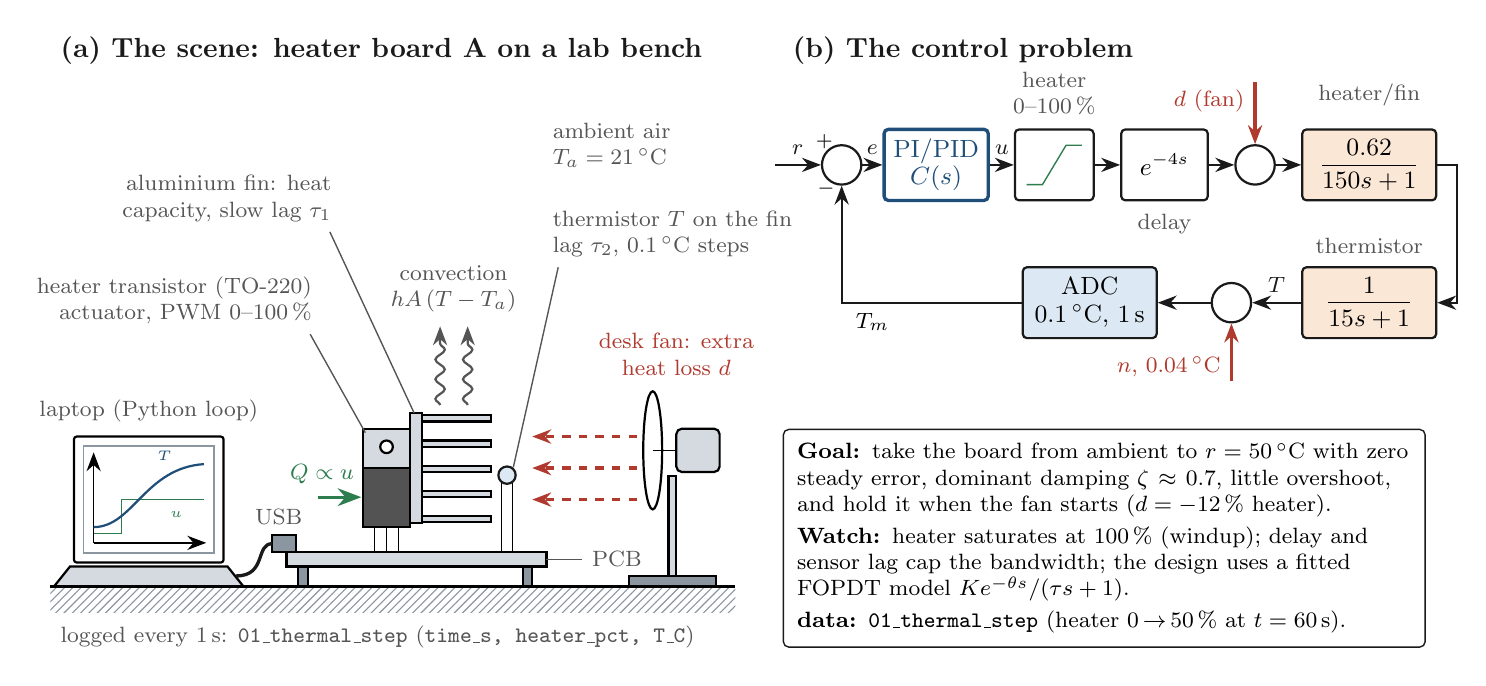
\begin{tikzpicture}
% ================= (a) the scene =================
\node[panel title] at (0,7.75) {(a) The scene: heater board A on a lab bench};
% bench
\fill[ground] (0,0.62) rectangle (8.7,0.95);
\draw[thick line] (0,0.95) -- (8.7,0.95);
\node[caption, anchor=west] at (0,0.3) {logged every 1\,s: \texttt{01\_thermal\_step} (\texttt{time\_s, heater\_pct, T\_C})};

% laptop (front view) with the logged signals on screen
\draw[fill=metal] (0.05,0.95) -- (2.45,0.95) -- (2.25,1.2) -- (0.25,1.2) -- cycle;
\draw[fill=white, rounded corners=1pt] (0.3,1.25) rectangle (2.2,2.85);
\draw[thin line, steel] (0.42,1.37) rectangle (2.08,2.73);
\draw[thin line, ->] (0.55,1.5) -- (1.98,1.5);
\draw[thin line, ->] (0.55,1.5) -- (0.55,2.65);
\draw[act, thin line] (0.55,1.62) -- (0.9,1.62) -- (0.9,2.05) -- (1.95,2.05);
\draw[accent] (0.55,1.7) .. controls (1.05,1.7) and (1.2,2.45) .. (1.95,2.5);
\node[font=\tiny, act, anchor=north] at (1.6,2.03) {$u$};
\node[font=\tiny, accent, anchor=south] at (1.45,2.42) {$T$};
\node[caption, anchor=south] at (1.25,2.9) {laptop (Python loop)};

% PCB on stand-offs
\foreach \x in {3.15,6.0} \draw[fill=steel] (\x,0.95) rectangle ++(0.12,0.25);
\draw[fill=metal] (3.0,1.2) rectangle (6.3,1.38);
\draw[thin line, note] (6.3,1.29) -- (6.75,1.29);
\node[caption, anchor=west] at (6.75,1.29) {PCB};
% USB connector and cable to the laptop
\draw[fill=steel] (2.82,1.38) rectangle (3.12,1.6);
\draw[thick line, ink] (2.82,1.49) .. controls (2.6,1.49) and (2.75,1.08) .. (2.36,1.08);
\node[caption, anchor=south] at (2.9,1.6) {USB};

% TO-220 heater transistor
\foreach \x in {4.12,4.27,4.42} \draw[thin line] (\x,1.38) -- (\x,1.7);
\draw[fill=ink!75] (3.97,1.7) rectangle (4.57,2.45);
\draw[fill=metal] (3.97,2.45) rectangle (4.57,2.95);
\draw[fill=white] (4.27,2.72) circle (0.08);
% aluminium fin bolted to the tab
\draw[fill=metal] (4.57,1.75) rectangle (4.72,3.15);
\foreach \y in {1.8,2.12,2.44,2.76,3.08}
  \draw[fill=metal] (4.72,\y-0.04) rectangle (5.6,\y+0.04);
% thermistor bead touching the fin tip, leads to the PCB
\draw[thin line] (5.73,2.3) -- (5.73,1.38);
\draw[thin line] (5.87,2.3) -- (5.87,1.38);
\draw[fill=sensorc, draw=ink] (5.8,2.36) circle (0.11);

% heat flow: electrical power into the transistor (actuation), fin -> air (losses)
\draw[force, act] (3.4,2.08) -- (3.95,2.08);
\node[act, anchor=south, font=\footnotesize] at (3.45,2.12) {$Q \propto u$};
\foreach \x in {4.95,5.3}
  \draw[->, note, decorate, decoration={snake, amplitude=0.6mm, segment length=2.5mm, post length=1.5mm}]
    (\x,3.25) -- (\x,4.25);
\node[caption, anchor=south, align=center] at (5.12,4.3) {convection\\$hA\,(T - T_a)$};

% labels with leader lines
\draw[thin line, note] (4.0,2.9) -- (3.3,4.15);
\node[caption, anchor=south east, align=right] at (3.45,4.15) {heater transistor (TO-220)\\actuator, PWM 0--100\,\%};
\draw[thin line, note] (4.62,3.15) -- (3.55,5.45);
\node[caption, anchor=south east, align=right] at (3.7,5.45) {aluminium fin: heat\\capacity, slow lag $\tau_1$};
\draw[thin line, note] (5.88,2.46) -- (6.45,5.0);
\node[caption, anchor=south west, align=left] at (6.25,5.0) {thermistor $T$ on the fin\\lag $\tau_2$, 0.1\,$^\circ$C steps};

% ambient
\node[caption, anchor=west, align=left] at (6.25,6.55) {ambient air\\$T_a = 21\,^\circ$C};

% desk fan (side view, blowing to the left)
\draw[fill=steel] (7.35,0.95) rectangle (8.45,1.08);
\draw[fill=metal] (7.85,1.08) rectangle (7.95,2.35);
\draw[fill=metal, rounded corners=2pt] (7.95,2.4) rectangle (8.5,2.95);
\draw[fill=white] (7.65,2.675) ellipse (0.12 and 0.75);
\draw[thin line] (7.65,2.675) -- (7.95,2.675);
\foreach \y in {2.05,2.45,2.85}
  \draw[distsig, dashed] (7.45,\y) -- (6.12,\y);
\node[caption, anchor=south, align=center, text=dist] at (7.95,3.5) {desk fan: extra\\heat loss $d$};

% ================= (b) the control problem =================
\begin{scope}[xshift=9.3cm]
\node[panel title] at (0,7.75) {(b) The control problem};
\def\yt{6.3} \def\yb{4.55}
\node[sum] (s1) at (0.75,\yt) {};
\node[font=\scriptsize] at ($(s1)+(-0.22,0.3)$) {$+$};
\node[font=\scriptsize] at ($(s1)+(-0.2,-0.3)$) {$-$};
\draw[sig] (-0.1,\yt) -- node[above, font=\footnotesize] {$r$} (s1);
\node[ctrl, minimum width=13mm] (C) at (1.95,\yt) {PI/PID\\[-1pt]$C(s)$};
\node[block, minimum width=10mm] (sat) at (3.45,\yt) {};
\draw[thin line, act] ($(sat)+(-0.35,-0.25)$) -- ($(sat)+(-0.15,-0.25)$) -- ($(sat)+(0.15,0.25)$) -- ($(sat)+(0.35,0.25)$);
\node[caption, anchor=south, align=center] at ($(sat)+(0,0.5)$) {heater\\0--100\,\%};
\node[block, minimum width=11mm] (del) at (4.85,\yt) {$e^{-4s}$};
\node[caption, anchor=north] at ($(del)+(0,-0.5)$) {delay};
\node[sum] (s2) at (6.0,\yt) {};
\node[plant, minimum width=17mm] (G1) at (7.45,\yt) {$\dfrac{0.62}{150s+1}$};
\node[caption, anchor=south] at ($(G1)+(0,0.62)$) {heater/fin};
\draw[sig] (s1) -- node[above, font=\footnotesize] {$e$} (C);
\draw[sig] (C) -- node[above, font=\footnotesize] {$u$} (sat);
\draw[sig] (sat) -- (del);
\draw[sig] (del) -- (s2);
\draw[sig] (s2) -- (G1);
\draw[distsig] (6.0,7.35) -- node[left, font=\footnotesize, dist, pos=0.3] {$d$ (fan)} (s2);
% bottom row (signals flow right to left)
\node[plant, minimum width=17mm] (G2) at (7.45,\yb) {$\dfrac{1}{15s+1}$};
\node[caption, anchor=south] at ($(G2)+(0,0.5)$) {thermistor};
\node[sum] (s3) at (5.7,\yb) {};
\node[sensor, minimum width=17mm] (adc) at (3.9,\yb) {ADC\\[-1pt]$0.1\,^\circ$C, 1\,s};
\draw[sig] (G1.east) -- ++(0.25,0) |- (G2.east);
\draw[sig] (G2) -- node[above, font=\footnotesize] {$T$} (s3);
\draw[sig] (s3) -- (adc);
\draw[distsig] (5.7,3.55) -- node[left, font=\footnotesize, dist, pos=0.25] {$n$, 0.04\,$^\circ$C} (s3);
\draw[sig] (adc) -- (0.75,\yb) -- (s1);
\node[font=\footnotesize, anchor=north west] at (0.8,\yb) {$T_m$};

% goal box
\node[draw=ink, thin line, rounded corners=2pt, fill=white, anchor=north west, align=left,
      text width=78mm, font=\footnotesize, inner sep=5pt] at (0,2.95) {%
  \textbf{Goal:} take the board from ambient to $r = 50\,^\circ$C with zero steady error,
  dominant damping $\zeta \approx 0.7$, little overshoot, and hold it when the fan starts
  ($d = -12\,\%$ heater).\\[2pt]
  \textbf{Watch:} heater saturates at 100\,\% (windup); delay and sensor lag cap the bandwidth;
  the design uses a fitted FOPDT model $K e^{-\theta s}/(\tau s+1)$.\\[2pt]
  \textbf{data:} \texttt{01\_thermal\_step} (heater 0\,$\to$\,50\,\% at $t = 60$\,s).};
\end{scope}
\end{tikzpicture}
\end{document}
